%! TeX root = ../charles/en/thesis.tex
\chapter{Datasets and Models}
\label{chap:dataset}

This chapter describes the existing datasets and models used in our experiments
in detail.  We first look at two video question answering datasets,
STAR~\citep{wu2021star} and NExT-QA~\citep{xiao2021nextqa}, and then discuss the
model we adapt for use in our experiments, Merlot
Reserve~\citep{zellers2022mreserve}. STAR is tested zero-shot in Merlot Reserve,
and achieves state of the art performance. In \cref{chap:method,chap:results}
we test how we can modify this model to improve its temporal reasoning ability,
while keeping strong performance on the STAR dataset. We further use NExT-QA to
test the generalisability of our model.
%TODO: Use NexT-QA ATP\textsubscript{hard} subset as well.

\section{STAR}

STAR~\citep{wu2021star} is a dataset for situated reasoning in real-world videos.
It uses videos taken from the Charades~\citep{sigurdsson2016charades} dataset,
which describe daily life actions or activities in indoor scenes. A video
is annotated with actions and timestamps. STAR builds a detailed scene annotation
from these videos. A situation is a description of entities, events, movements,
and environments. An example is shown in \cref{fig:star}.

\begin{figure}[htpb]
	\centering
	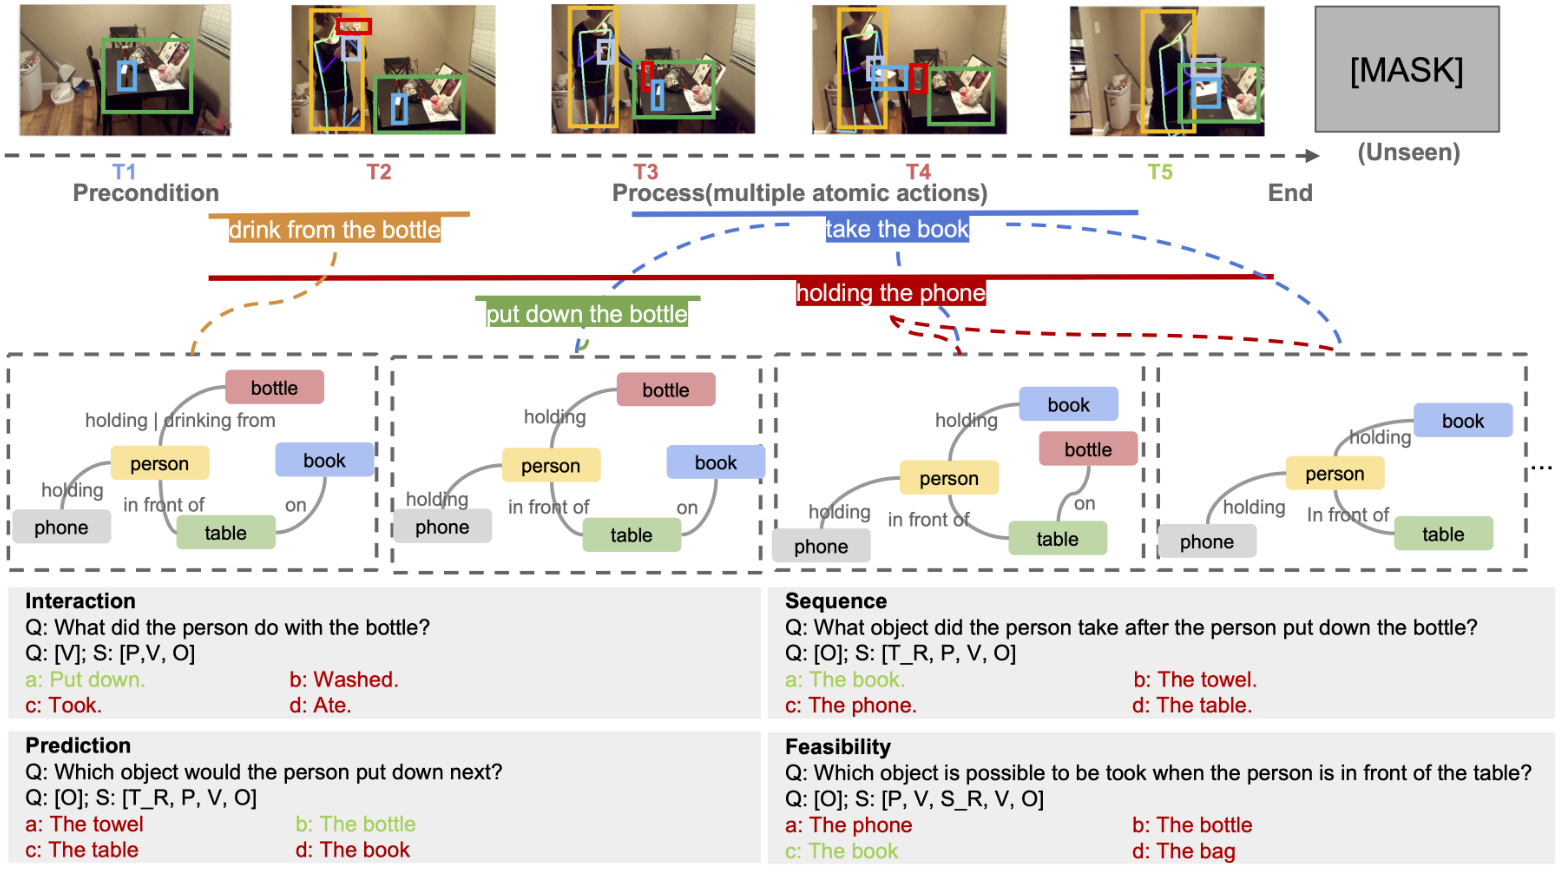
\includegraphics[width=0.8\textwidth]{star}
	\caption{An example instance from the STAR dataset, with the four question
		types. Image from~\citet{wu2021star}}
	\label{fig:star}
\end{figure}

There are four types of question: interaction, sequence, prediction, and
feasibility.  Based on the type of question, a situation will include complete
action segments or, for prediction and feasibility questions, involve actions
involved in the questions and an incomplete action segment about answers.
Answers are generated to provide three different distractors along with the
correct answer. The compositional distractor satisfies verb-object
compositionality and is generated so as to be feasible in the same situation.
The random option is selected from other instances, with the constraint that
compositionality is satisfied, while the frequent option selects the most
frequently occurring answer in each type of question group to deceive models
that look for shortcuts in this way.

With respect to temporal reasoning, of particular interest to us are the
sequence questions. These are questions which evaluate the temporal reasoning
of systems when facing consecutive actions in dynamic situations, and ask about
relationships between people and objects through the actions they perform in a
situation. The best baseline model achieves an average accuracy of 36.7\%
across all question types. In their baseline results, the authors note that
visual perception has a significant impact on situated reasoning. Existing
vision models struggle to reason well in real-world situations, and models
struggle more to identify relationships between objects than objects
themselves. It is therefore the task of an improved video and language model to
better realise these relationships.

\section{NExT-QA}

%Description. Explanation of temporal questioning. Used for evaluation in different domain
NExT-QA~\citep{xiao2021nextqa} is another video question answering dataset with
a focus on a wider range of temporal actions. Where STAR asks questions that
test only before/after temporal relations, questions in NExT-QA challenge the
model to reason about causal actions as well as temporal relations such as
`when` (\cref{fig:nextqa}).

\begin{figure}[htpb]
	\centering
	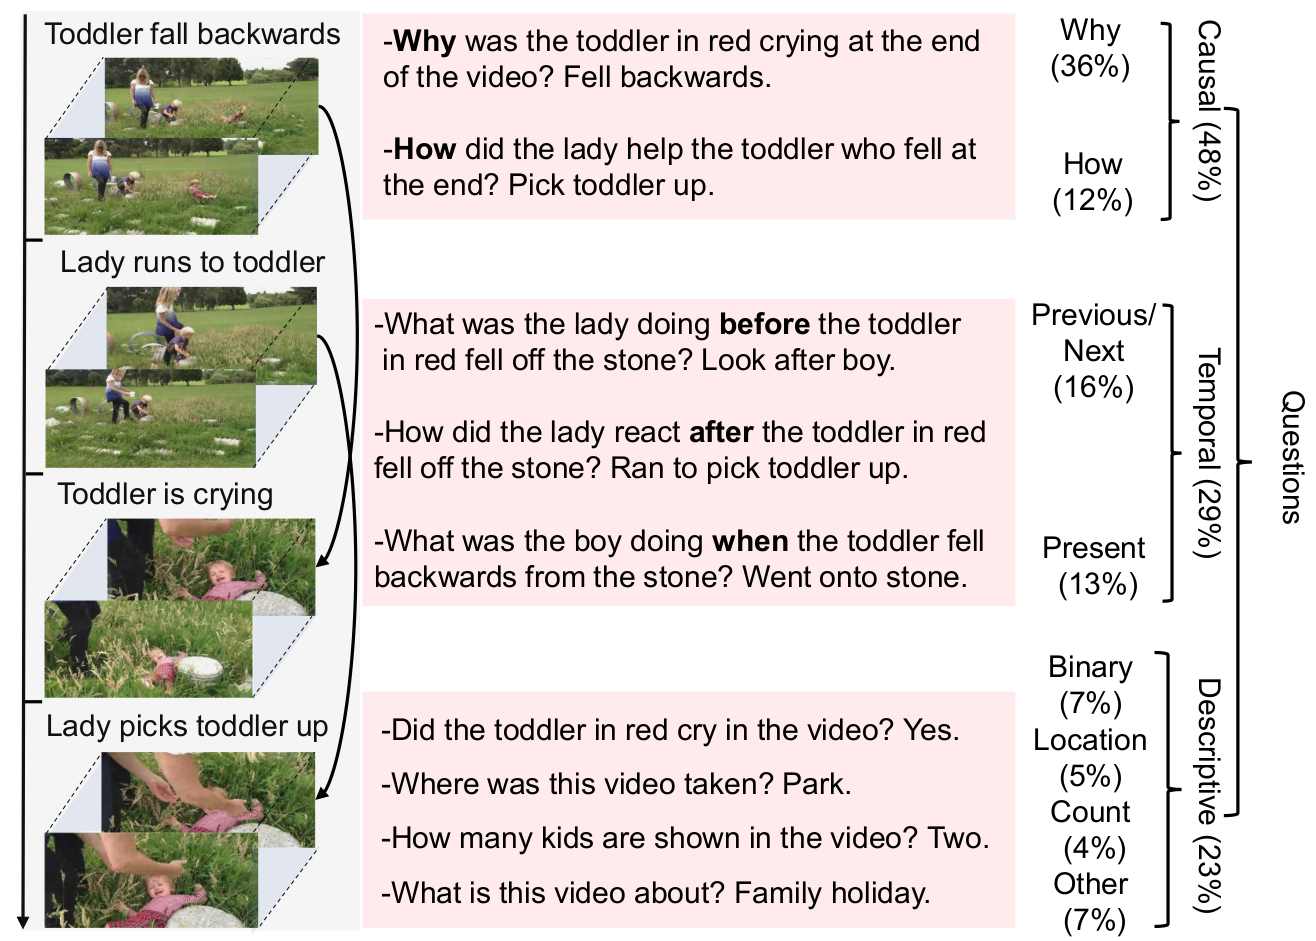
\includegraphics[width=0.8\textwidth]{nextqa}
	\caption{Example NExT-QA video and question types.
		From~\citet{xiao2021nextqa}}
	\label{fig:nextqa}
\end{figure}

\section{Merlot Reserve}

Merlot Reserve~\citep{zellers2022mreserve} is a pre-trained video language model
which uses a contrastive objective that learns from aligned audio, subtitles
and video frames. The authors collect a diverse dataset of 1 billion frames
from YouTube videos. Videos are filtered to be high quality, favouring
instructional videos so that there would be a visual grounding to the subtitles
and audio. The architecture consists of independent encodings of each modality,
via a Vision Transformer~\citep{dosovitskiy2021vit}, an Audio Spectrogram
Transformer~\citep{gong2021ast}, and a Transformer span encoder, which computes
targets from an embedding of a candidate text span
(\cref{fig:mreservearch}). This is then fed into a joint Transformer encoder
for all modalities and timesteps.

The specific pre-training objective is called contrastive span training
(\cref{fig:contrastivespan}). For each frame aligned with an image, text,
and audio encoding, a region of text and audio is masked out. The model must
maximise its similarity only to an independent encoding of the text and audio.
In pre-training the model learns to predict spans of text and audio in two
cases: predicting audio where frames and text is provided; and predicting text
where frames and audio are provided. 

\begin{figure}[htpb]
	\centering
	\begin{subfigure}[b]{0.45\textwidth}
		\centering
		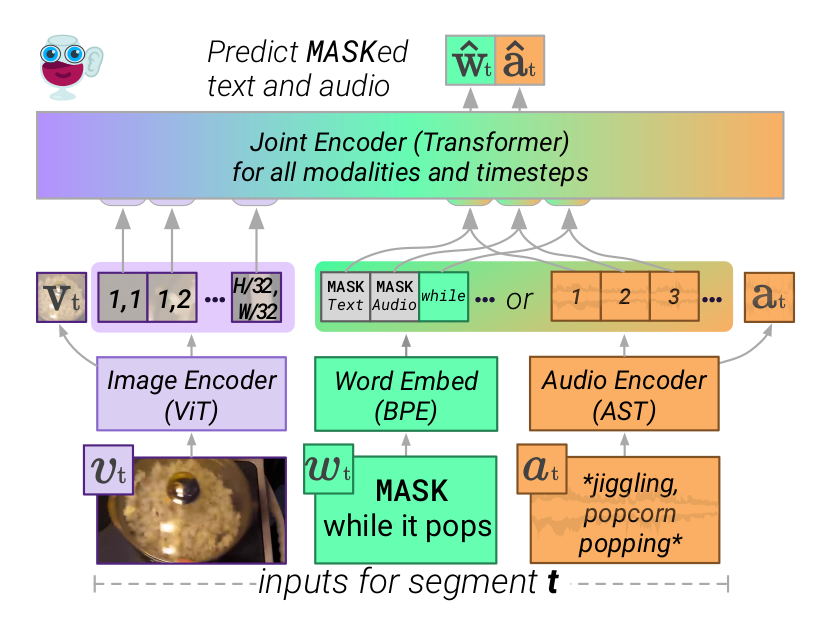
\includegraphics[width=\textwidth]{mreservearch}
		\caption{Merlot Reserve Architecture}
		\label{fig:mreservearch}
	\end{subfigure}
	\hfill
	\begin{subfigure}[b]{0.45\textwidth}
		\centering
		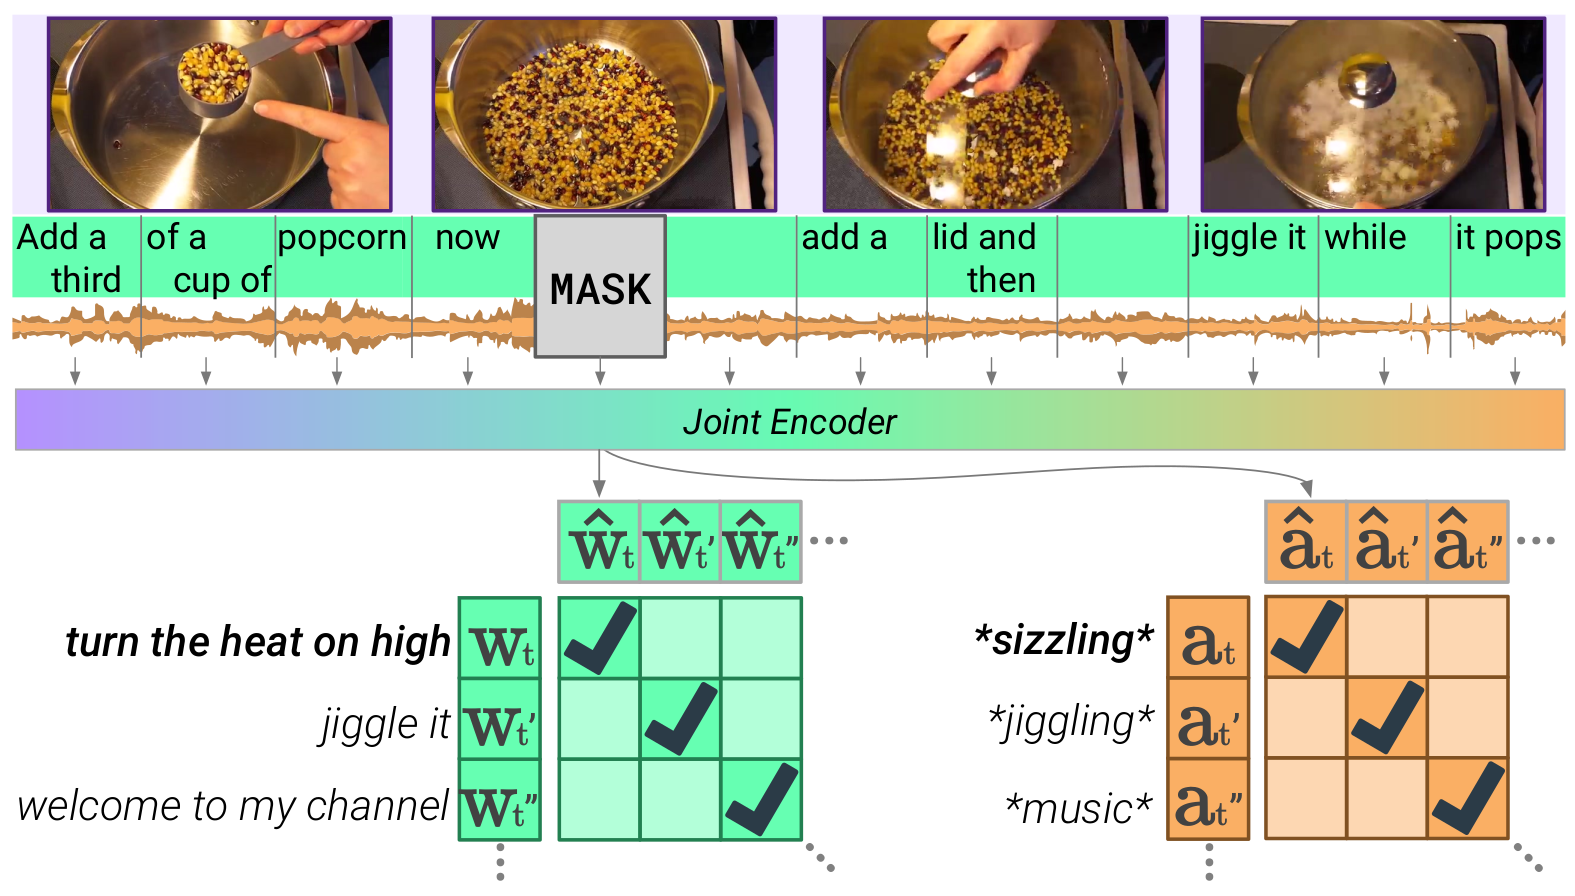
\includegraphics[width=\textwidth]{contrastivespan}
		\caption{Contrastive Span Training}
		\label{fig:contrastivespan}
	\end{subfigure}
	\caption{Merlot Reserve Details. Figures taken from~\citet{zellers2022mreserve}}
	\label{fig:mreserve}
\end{figure}

Once pre-trained, the model can be used by finetuning on a dataset, or
zero-shot for a range of video and language tasks. The authors achieved state
of the art results on visual commonsense reasoning~\citep{zellers2019vcr},
TVQA~\citep{antol2015vqa}, another video question answering dataset, and
Kinetics-600~\citep{carreira2018kinetics600}, for activity understanding.
Further, zero-shot experiments showed performance competing with those of
supervised models on a range of video question answering datasets, and even
slightly exceeding the supervised state of the art on STAR.
